\chapter{Einleitung}

Das 6. Semester der Hochschule Furtwangen beinhaltet f�r den Studiengang Elektronik und Technische Informatik (ETI) die M�glichkeit durch Wahlpflicht Vorlesungen (WPVs) das gesamt Bild des angehenden Engineers abzurunden.

Gerade f�r einen Elektrotechniker bietet es sich daher an, nicht nur die Elektrotechnische-Welt zu kennen, sondern auch die unz�hligen M�glichkeiten der Informatik kennen zu lernen, und diese in Kombination zu nutzen.

Aus diesem Gedanken heraus ist die Idee entstanden ein Programm mit C\# zu entwickeln, welches den Arbeitsalltag eines Elektrotechnikers enorm erleichtern kann, indem regelungstechnische Auslegungen schnell und komfortabel durchgef�hrt werden k�nnen.

Um beide Welten sauber in Einklang bringen zu k�nnen wird auf der Elektrotechnischen Seite auf die Regelungstechnik mit der Laplace-Transformation und die Z-Transformation zur�ck gegriffen und auf der Informatik Seite auf die Vorz�ge der Objektorientierten Programmiersprache C\# und die Verwendung von "`Design Patterns"'.

%---------------------------------------------------------
\section{Wichtiges �ber die Regelungstechnik}
\begin{description}

\item \textbf{Warum Regelungstechnik?}

In sehr vielen Anwendungen kommt es vor, dass man einen soll-Wert vorgibt, und diesen mit einem ist-Wert vergleicht und dann entscheidet was gemacht werden soll. Dieser Vorgang wird in der Regelungstechnik behandelt.

So kann man sich z.B. vorstellen, dass ein Motor auf eine gewisse soll-Drehzahl beschleunigt werden soll. Da die Drehzahl sich wegen der Tr�gheit der Masse des Motors nicht direkt auf die gew�nschte Drehzahl begibt, wird ein Regler eingesetzt. Dieser schaut sich den Soll-Ist Vergleich an und entscheidet dann, ob entweder \textit{mehr Drehmoment} oder \textit{weniger Drehmoment} aufgebracht werden muss, um den Motor auf die gew�nschte Drehzahl zu bringen.

\begin{figure}[H]
	\centering
  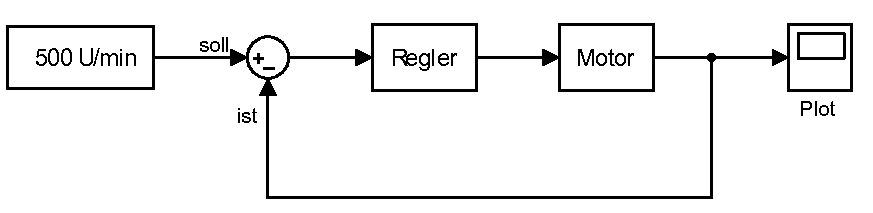
\includegraphics[width=1\textwidth]{Bilder3/Motor_Regelkreis.pdf}
	\caption{Beispiel Regelkreis f�r einen Motor}
	\label {Beispiel Regelkreis f�r einen Motor}
\end{figure}

In der Regelungstechnik werden nun verfahren untersucht, um diesen Regler ideal einzustellen, damit dass zeitlich dynamische Verhalten eines Vorgangs ideal in den Griff gebracht werden kann.


\item \textbf{Was sind �bertragungsfunktion?}

Um dynamische Vorg�nge in der Physikalischen Welt Mathematisch beschreiben zu k�nnen werden in der Regel so genannte Differentialgleichungen eingesetzt.
Hierdurch kann z.B. das dynamische Verhalten eines Motors, einer elektronischen Schaltung, einer Temperatur,eines mechanischen Vorgangs, ... beschrieben werden.

Das eigentlich Problem besteht nun oft darin, dass das l�sen dieser Differentialgleichnung sehr schwer ist. 
An dieser Stelle bietet die Laplace-Transformation einen eleganten Weg, um aus einer Differentialgleichung eine �bertragungsfunktion im Laplace-Bereich zu gewinnen.

Diese �bertragungsfunktion (Transferfunktion) bietet f�r unsere Zwecke entscheidende Vorteile:

\begin{itemize}
	\item \textit{Handhabung}
	
	Es ist wesentlich einfacher mit einer �bertragungsfunktion zu rechnen.
	\item \textit{Universell}
	
	Die Regelungstechnik ist f�r alle dynamischen Vorg�nge equivalent!
	\item \textit{Simulierbar}
	
	Durch Verwendung der Z-Transformation kann eine �bertragungsfunktion "`relativ"' einfach auf einem Computer Simuliert werden.
	\item \textit{Betrachtung als Block}
	
	Die einzelnen �bertragungsfunktionen f�r Regler, Motor, ... k�nnen als Bl�cke wie in Bild\vref{Beispiel Regelkreis f�r einen Motor} betrachtet werden.
\end{itemize}

\newpage
\item \textbf{Warum ein extra Software Tool?}

Die gesamte Regelungstechnik besteht zum gr��ten Teil aus Mathematik. Hier kann es sehr schnell passieren, dass man den �berblick verliert, da es einem schwer f�llt gewisse abstrakte Gebilde sich vorzustellen. 

Das hier entwickelte Software Tool m�chte genau an dieser Stelle ans�tzen, dem Benutzer ein Gef�hl daf�r zu geben, wie die einzelnen abstrakten Gebilde zusammen h�ngen, und welchen Einfluss die einzelnen Parameter auf das dynamische Verhalten des Systems haben.

Dar�ber hinaus sind bereits verfahren hinterlegt, um einen Regler gut auszulegen, und diesen visuell in Echtzeit an die Bed�rfnisse des Engineers nach tunen zu k�nnen.
Aus diesem grund hat das neu entstandene Tool den Namen "`Live-Tuner"' erhalten.

\end{description}